\chapter{Ecologically valid objective evaluation of Hearing Aids and DNN-based binaural Speech Enhancement}
\chaptermark{Evaluation of Hearing Aids}
\label{ch03_hearing}

Hearing aids (\acrshort{HAs}) are the primary clinical remedy for hearing
loss. Beyond restoring audibility through frequency-dependent amplification
and dynamic range compression, their practical value rests largely on a
harder problem: keeping speech intelligible amid competing sounds. To improve
the \acrfull{SNR}, hearing aids traditionally rely on directional microphones
\citep{ricketts1999} and adaptive beamformers
\citep{luo2002adaptive, gode2022}, complemented by single-channel
noise reduction. This enhancement is typically validated with stationary
noises under controlled laboratory conditions \citep{IEC6011816}. Everyday
listening, however --- a party, a restaurant, several competing talkers --- is
non-stationary and spatially complex, precisely the regime these methods
handle worst. The resulting mismatch between the conditions under which a
device is \emph{evaluated} and those in which it is \emph{used} is a question
of ecological validity, and closing it for hearing aids is the aim of
\textbf{RO1}.

In parallel, end-to-end \acrshort{DNN}s (Section~\ref{sec:bg_dl}) have
transformed speech enhancement, achieving strong denoising even in the
monaural case \citep{reddy2021icassp}. Their adoption in hearing devices has
been constrained by the requirement of causality and by tight compute and
latency budgets, but both are eroding: causal architectures have been
proposed \citep{tzinis2020sudo} and scaled \citep{ali2023scaling}, binaural
models preserve spatial cues \citep{han2020}, algorithmic latencies now
approach those of conventional hearing-aid processing
\citep{wang2023neural, stone2008delays}, and network miniaturisation
\citep{banbury2021micronets}, computation offloading \citep{sun2020supervised}
and the Clarity Challenge \citep{clarity} together make \acrshort{DNN}-based
hearing-aid enhancement increasingly plausible. Indeed, some manufacturers
already embed \acrshort{DNN} post-filtering in commercial products
\citep{andersen2021, oticon2, oticon3}, yet without disclosing their
architectures or any ablation quantifying the gain they bring. Whether
\acrshort{DNN}s genuinely generalise better than the mature, hand-engineered
enhancement of current devices, especially in the complex scenes where the
latter struggle, is therefore an open question and the object of
\textbf{RO2}.

This chapter, the result of a collaboration with Microson (Amplifon Group),
addresses both objectives with a single evaluation setup. \textbf{We
record five high-end commercial hearing aids exposed to complex
speech-in-noise scenes, reproduced over an Ambisonic loudspeaker array and captured on a \acrshort{KU100} dummy head,
and we compare their built-in enhancement against the same recordings
post-processed by two state-of-the-art \acrshort{DNN}s}. 

The main contribution
is an evaluation which suggests that \acrshort{HAs} traditional enhancement
struggles under challenging acoustic conditions, and that \acrshort{DNN}-based
\acrshort{SE} has the potential to improve current hearing devices.
Along the way, and helping to fill the absence of any public hearing-aid
evaluation dataset noted in Chapter~\ref{ch02_sota}, we release an
Ambisonics-to-binaural decoder tailored to a hearing aid, a synthetic
binaural training corpus, and a reverberant speech-in-noise test set with the
corresponding recordings of each device.

\section{Hearing Aids Measurement Setup}
\label{sec:ha_setup}

We first describe the measurement and evaluation infrastructure, deferring the
enhancement strategies it serves to compare --- both the conventional
hearing-aid processing and the \acrshort{DNN}-based enhancement --- to
Section~\ref{sec:ha_dnn}. The purpose here is only to explain how ecologically
valid scenes are generated, reproduced, captured on the hearing devices, and
turned into signals amenable to objective evaluation.

\subsection{Overview}
\label{sec:ha_overview}

The setup, depicted in Figure~\ref{fig:ha_setup}, was designed to capture the
signals a hearing device actually processes within complex acoustic scenes,
and comprises three stages. In \emph{scene generation}, realistic
speech-in-noise scenes are built by combining existing databases with
room-acoustic simulation, and rendered as Ambisonic sound fields. In
\emph{recording}, these scenes are reproduced over an Ambisonic loudspeaker
array and captured with the microphones of a dummy head wearing each hearing
aid, with and without the device's enhancement features. In \emph{evaluation},
the hearing-aid-enhanced recordings are compared against the same signals
processed by the \acrshort{DNN}s, using a set of objective metrics computed
against a clean binaural reference. The following subsections detail each
component of this pipeline.

\begin{figure}[htbp]
  \centering
  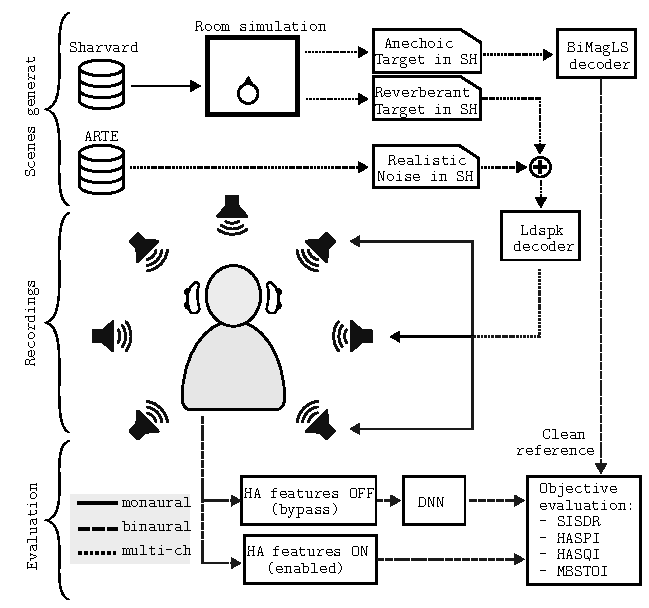
\includegraphics[width=0.8\columnwidth]{ch03_hearing/figures/waspa01.pdf}
  \caption{Hearing-aid measurement setup. \emph{Scene generation}: complex
  acoustic scenes are created by combining existing databases (Sharvard,
  ARTE) with room-acoustic simulation. \emph{Recording}: the material is
  played back over an Ambisonic reproduction system and the signals processed
  by the hearing aid are captured with the microphones of a dummy head, with
  and without its signal-enhancing features. \emph{Evaluation}: the
  hearing-aid-enhanced recordings are compared with the \acrshort{DNN}-processed
  ones through a range of objective metrics.}
  \label{fig:ha_setup}
\end{figure}

\subsection{Ambisonic complex-scene generation}
\label{sec:ha_scenes}

To ensure that the sound reaching each device closely resembled real life, all
scenes were represented and reproduced as Ambisonic sound fields
(Section~\ref{sec:bg_spatial}). We built three acoustic scenes of speech in
noise, corresponding to three common environments: \emph{party},
\emph{restaurant} and \emph{office}. The noise came from the \acrfull{ARTE} database \citep{weisser2019ambisonic},
whose recordings were captured in real environments with a 62-channel
microphone array and distributed as 31-channel \emph{mixed-order} Ambisonics.

In a mixed-order representation the horizontal plane is encoded at a higher
spherical-harmonic order than the vertical one, exploiting the fact that both
most sources and human localisation are concentrated near the horizontal:
full-sphere resolution is kept only up to a low order, and the
additional horizontal detail is carried by the sectorial harmonics
($m=\pm\ell$, the outermost components of the harmonic pyramid in
Figure~\ref{fig:spherical_harmonics}) alone. \acrshort{ARTE} keeps the full
3D field up to 4th order (25 channels) and adds horizontal-only components up to 7th order (6 further channels), for 31 in total. We
zero-padded these into a full 10th-order set, placing each component in its
ACN slot and filling the remaining, unmeasured harmonics with
zeros. The target
speech consisted of nine sentences spoken by a female speaker, drawn from the
phonemically balanced Spanish Sharvard corpus \citep{aubanel2014shavrvard}.

Room acoustics were simulated with an adaptation of the \acrfull{MASP} library\footnote{\url{https://github.com/andresperezlopez/masp}}, a shoebox \acrshort{ISM} simulator (Section~\ref{sec:bg_rir_ism})
extended to output the field directly in Ambisonics domain. \acrshort{MASP} is the translation from \cite{politis2016microphone}'s MATLAB library into Python \citep{perez2020parametric}. Working at 10th order, which affords sufficient spatial
resolution, we simulated for each scene two sound fields at the left-ear,
right-ear and \emph{head} positions: an anechoic one, propagating only the
direct sound, and a reverberant one. The two ear positions were placed
$17.5\,\text{cm}$ apart to match the \acrshort{KU100} inter-ear distance. The
three rooms measured $15\times10\times3.5\,\text{m}$,
$28\times17\times4.2\,\text{m}$ and $5\times2\times2.5\,\text{m}$ for the
\emph{party}, \emph{restaurant} and \emph{office} scenes respectively, and the
target was placed $1\,\text{m}$ from the head at either $0^{\circ}$ or
$30^{\circ}$ to the right. The reverberation times were set by informal
listening against the \acrshort{ARTE} recordings, choosing $T_{60}$ values
around $60\%$ of those reported for \acrshort{ARTE} to account for the
absorption of furniture and people. The result is a set of clean (anechoic)
and reverberant speech and noise fields, all in Ambisonics.

\subsection{Decoding to the loudspeaker array}
\label{sec:ha_lsdecoding}

Playback took place in Eurecat's Spatial Audio recording and mixing studio, a three-dimensional
irregular array of 25 Genelec 8040 loudspeakers surrounding the listening
position. The studio is acoustically treated to keep its own reverberation short, but
it is not anechoic (Figure~\ref{fig:eurecat_studio}). The signals captured at the
dummy head therefore contain, on top of the reverberation deliberately
simulated into each scene, the small residual response of the playback room
itself; the acoustic treatment ensures this residual contribution stays well
below the intended, simulated acoustics that dominate the reproduced field. To reproduce a scene, the speech and noise sound fields were first
mixed at the \emph{head} position, weighting the two so that the binaural
signal-to-noise ratio was $+5\,\text{dB}$ once decoded to the ears (the
binaural decoder of Section~\ref{sec:ha_bindecoder}). The resulting Ambisonic
mixture was then decoded to the 25 loudspeaker feeds with a fifth-order
in-phase decoder (Section~\ref{sec:bg_ambi_timeline}) optimised with IDHOA
\citep{scaini2014decoding} for this particular irregular layout; the in-phase
design suppresses the side lobes of the virtual microphones, trading angular
sharpness for robustness away from the centre. Finally, all sets of
loudspeaker signals were normalised to equal energy to ease calibration.

\begin{figure}[htbp]
  \centering
  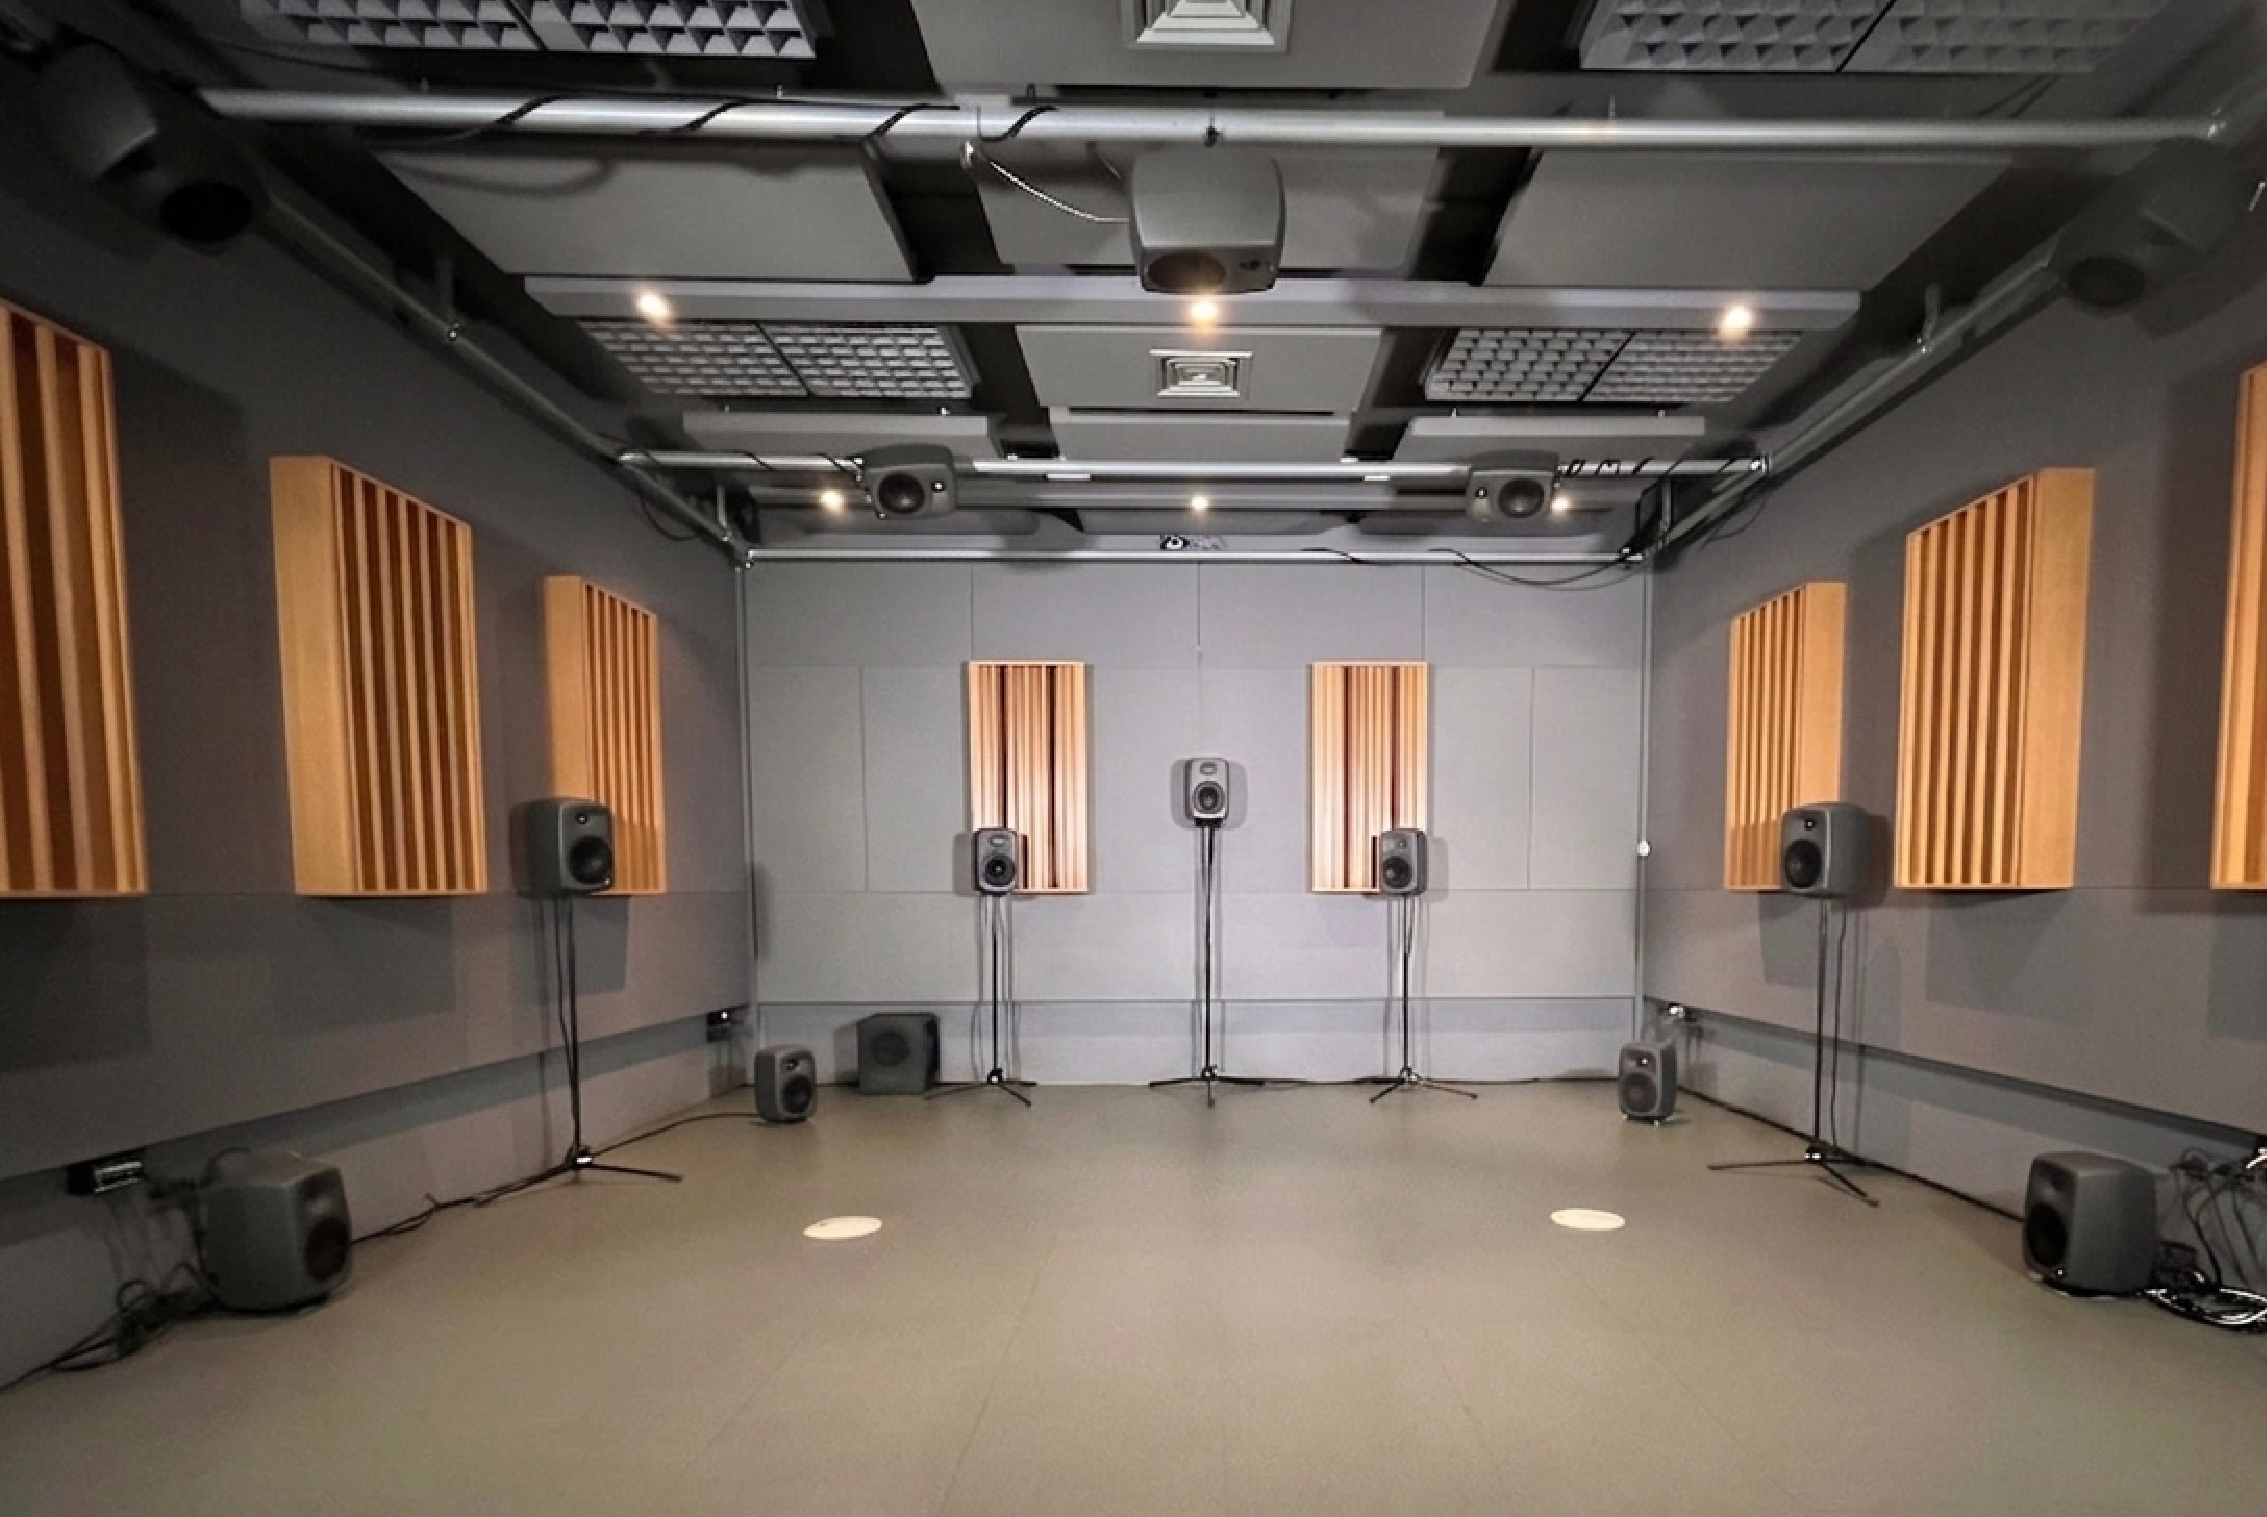
\includegraphics[width=\columnwidth]{ch03_hearing/figures/eurecat_studio.pdf}
  \caption{Eurecat's Spatial Audio studio: a three-dimensional irregular array of 25 Genelec 8040
  loudspeakers arranged in floor, ear level and
  ceiling.}
  \label{fig:eurecat_studio}
\end{figure}

\subsection{Dummy-head recordings}
\label{sec:ha_recordings}

A Neumann \acrshort{KU100} dummy head was placed at the centre of the array.
Each scene was
calibrated to $70\,\text{dB}$ \acrshort{SPL} at the ear position, next to the dummy head, using a
Beyerdynamic MM1 omnidirectional measurement microphone
(Figure~\ref{fig:ha_dummyhead}). We recorded five high-end \acrfull{RIC}
\acrshort{HAs} available on the market at the time of writing --- the GN ONE
961-DRWC and 561-DRWC, the Phonak Audéo P90-R and P70-R, and the Signia Pure
C\&G 3x --- testing fifteen \acrshort{HAs}–receiver combinations in total, with
low, mid and high-power receivers for each device. For each recording, the
\acrshort{HAs} were fitted behind the ears of the \acrshort{KU100} and their receivers
inserted into its ear canals; to minimise the contribution of direct sound
leaking past the device, the ear-canal entrance was occluded with adhesive
putty in addition to the \acrshort{HAs}' own power dome. Each scene was recorded twice with every \acrshort{HAs}. In the first pass the
device was set to \emph{bypass}: all signal-enhancing algorithms were
deactivated, leaving only the feedback canceller and a linear amplification of
approximately $20\,\text{dB}$. Since commercial devices offer no direct access
to their microphone signals, these \emph{bypass} recordings at the
\acrshort{KU100} serve as an approximation of what the hearing-aid microphones
capture, and are therefore also the input fed to the offline
\acrshort{DNN}-based enhancement of Section~\ref{sec:ha_dnn}. In the second
pass the device was set to \emph{enabled}, applying the signal-enhancement
algorithms of its default factory settings, which in all tested devices
included at least some form of adaptive beamforming and single-channel noise
reduction. No hearing correction was applied in either mode.

\begin{figure}[hb]
  \centering
  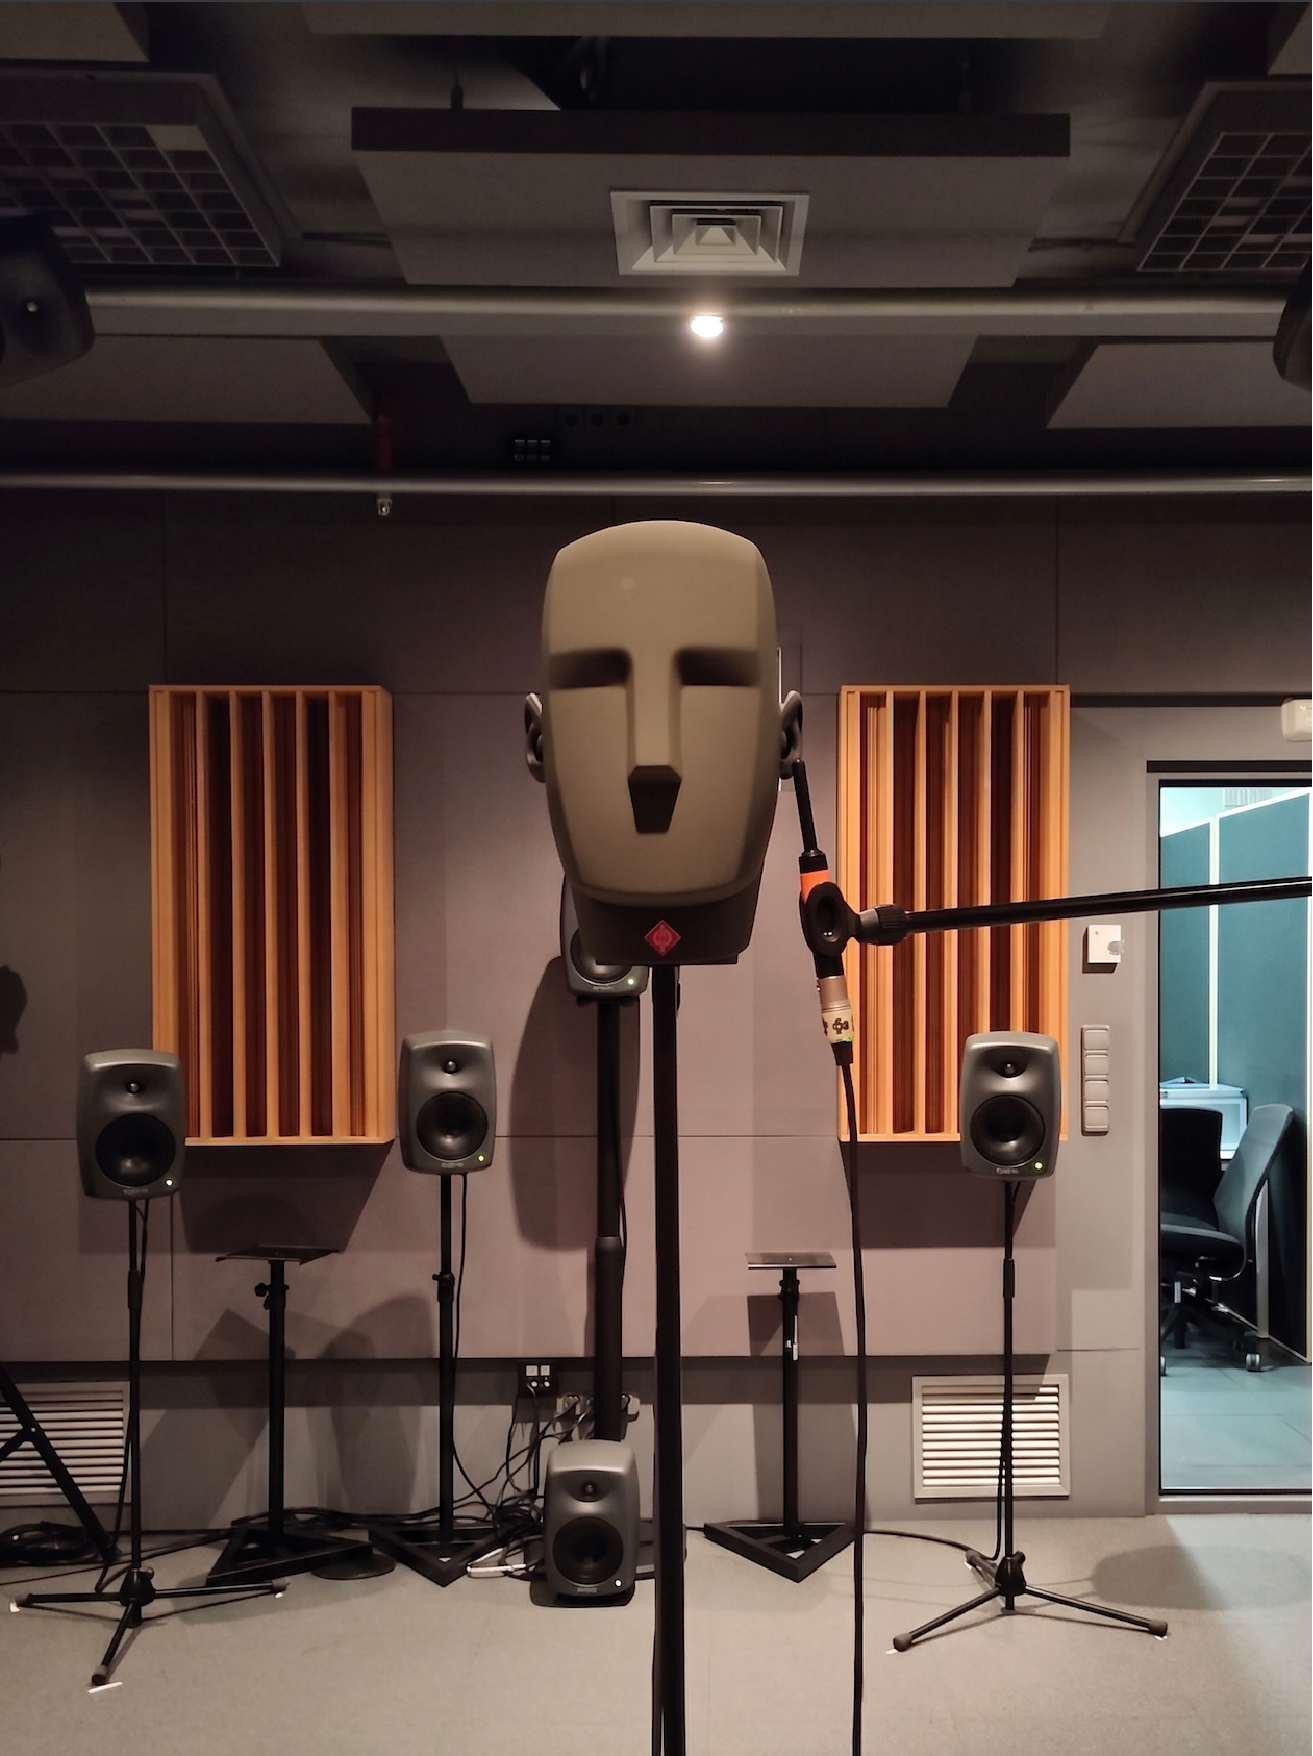
\includegraphics[width=0.6\columnwidth,trim={0cm 6cm 0cm 6cm},clip]{ch03_hearing/figures/ku100.pdf}
  \caption{The Neumann \acrshort{KU100} dummy head at the centre of the
  loudspeaker array, ready for calibration with the Beyerdynamic MM1 measurement microphone.}
  \label{fig:ha_dummyhead}
\end{figure}

\subsection{Ambisonics-to-binaural hearing-aid decoder}
\label{sec:ha_bindecoder}

Returning to the evaluation pipeline of Figure~\ref{fig:ha_setup}, the one
element missing before being able to evaluate the performance is a way to obtain the clean references against which the
metrics are computed. The intrusive metrics below require a clean binaural
reference matching what the hearing-aid microphones would capture in the
absence of noise and reverberation. Since our scenes live in the Ambisonic
domain --- including the anechoic speech field simulated in MASP
(Section~\ref{sec:ha_scenes}) --- obtaining that reference amounts to decoding
Ambisonics to binaural, which in turn calls for a set of \acrshort{HRTF}s
specific to the device-on-head configuration. Although \citet{oldenburg}
published \acrshort{HRTF}s for the microphones of a behind-the-ear hearing aid
on a head-and-torso simulator, none were available for the \acrshort{KU100},
and, evaluating commercial devices, we had no access to their microphone
signals. We therefore measured our own \acrshort{HRTF}s in a configuration as
close as possible to the recording setup: in the same room, with a pair of
\emph{audifon lewi R} hearing aids coupled to the dummy-head ear canals,
enhancement features disabled and only a linear gain applied.

The \acrshort{HRTF}s were measured with the exponential-sweep method
(Section~\ref{sec:bg_rir_sweep}) using a single Genelec 8020 loudspeaker
positioned at each of the 50 directions of a \emph{Lebedev grid}
(Figure~\ref{fig:lebedev}). Lebedev grids are sets of directions distributed as evenly as possible over
the sphere, arranged so that each one has its mirror image across every axis.
This symmetry covers all directions uniformly with comparatively few points:
the 50 directions comprise the $6$ vertices of an octahedron, the $8$ vertices
of a cube, the $12$ edge midpoints between them, and a further symmetric
orbit of $24$ points. Grouped by elevation, they form horizontal rings whose
population grows towards the horizontal plane --- a single point at each pole,
four at intermediate elevations and eight on the rings nearest and on the
horizontal --- since the rings near the equator are longer circles and fit
more points at an even spacing. This concentrates angular resolution around
the horizontal plane, where human localisation is most acute. Such efficiency
is convenient for \acrshort{HRTF} acquisition, where every added direction
means another physical measurement.

\begin{figure}[t]
  \centering
  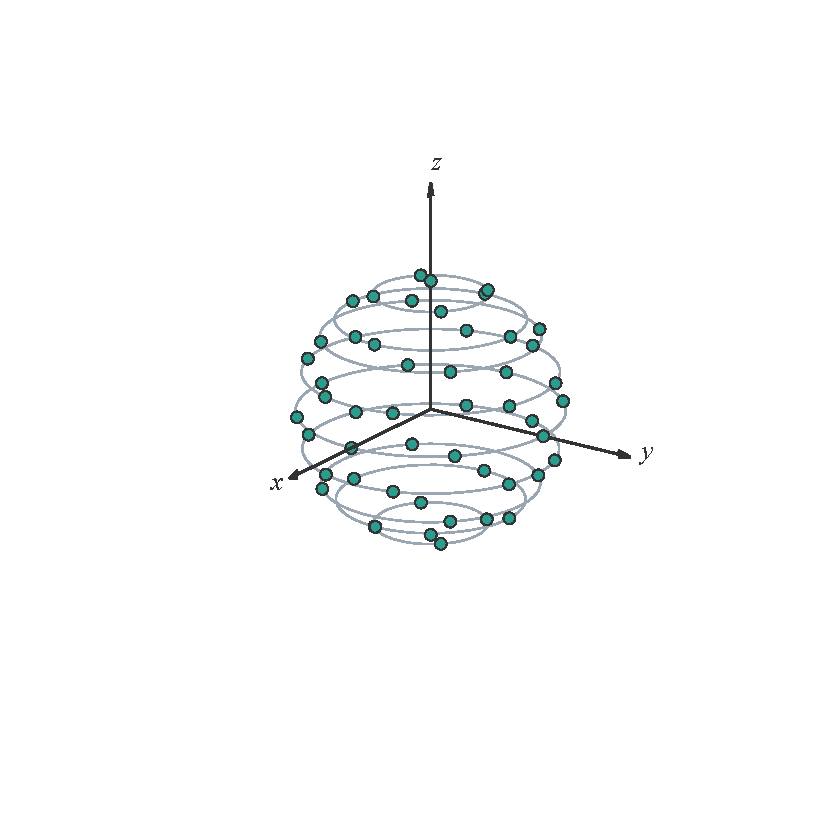
\includegraphics[width=.7\columnwidth,trim={4cm 4cm 3cm 2.5cm},clip]{ch03_hearing/figures/lebedev.pdf}
  \caption{The 50-point Lebedev grid of \acrshort{HRTF} measurement
  directions, shown on the unit sphere. The points group into horizontal rings
  of constant elevation: a single point at each pole, four at the intermediate
  elevations, and eight on the rings nearest and on the horizontal plane ---
  so the angular sampling is densest around the horizontal, where localisation
  matters most. Its octahedral symmetry yields this near-uniform,
  well-conditioned coverage from only 50 directions.}
  \label{fig:lebedev}
\end{figure}

The measured impulse responses were windowed before the arrival of the first
wall reflection, yielding quasi-anechoic responses, and their low-frequency
content was extended with the spherical-model \acrfull{LFE} of
\citet{bernschutz2013spherical}. From these we built a 10th-order
Ambisonics-to-binaural decoder following the \acrshort{BiMagLS} method~\citep{engel2021improving} (Section~\ref{sec:bg_ambi_timeline}), with
spherical-harmonic tapering above a cutoff of $6239\,\text{Hz}$ --- the
theoretical limit for correct representation at 10th order. The clean binaural
reference is then obtained by decoding, with this same decoder, the anechoic
left and right-ear sound fields simulated in \acrshort{MASP}.

The measured \acrshort{HRTF}s are released in the \acrfull{SOFA} format
\citep{aes69}. \acrshort{SOFA}\footnote{we used the Python library from \url{https://github.com/Jencke/pySOFA}}, standardised as AES69, is a self-describing container that stores acoustic impulse responses --- here the
\acrshort{HRIR} pairs --- together with the full measurement geometry (source
and receiver positions and orientations) and metadata, so that a dataset can
be exchanged and reused across tools without ambiguity. We provide both this
\acrshort{SOFA} file and the resulting \acrshort{BiMagLS} decoder as research
materials \footnote{\url{https://github.com/enricguso/guso_waspaa23}}.

\subsection{Evaluation metrics}
\label{sec:ha_metrics}

The objective evaluation compares four sets of recordings: \emph{bypass},
\emph{enabled}, \emph{bypass} post-processed with the non-causal model (\textbf{\acrshort{DNN}}) and  and \emph{bypass} post-processed with its causal counterpart (\textbf{\acrshort{DNN}-C}). The first
represents the absence of signal enhancement and the remaining three the
different enhancement strategies under comparison. 

In a preliminary round we attempted to estimate the output \acrshort{SNR} with
the phase-inversion procedure of \citet{hagerman2004method}. The idea is to
present the same scene twice: first the mixture of speech and noise, and then
the same mixture with the \emph{noise inverted in polarity}. If the device
applies the same processing in both passes, adding the two recordings cancels
the noise and leaves twice the processed speech, while subtracting them
cancels the speech and leaves twice the processed noise. Having isolated the
two components at the output, the output \acrshort{SNR} --- and hence the
improvement over the input --- follows directly. The procedure, however,
assumes that the system behaves identically across the two presentations; this
did not hold for several hearing aids, whose adaptive processing reacted
differently to the polarity-inverted noise, nor for any of the
\acrshort{DNN}s, whose non-linear mapping breaks the assumption outright,
making the estimates unreliable. We therefore relied on
intrusive, reference-based metrics computed against the clean binaural
reference $y$ of Section~\ref{sec:ha_bindecoder}. 

Given an enhanced estimate
$\tilde{y}$ and the corresponding unprocessed recording $\hat{y}$, we
time-aligned each pair to the reference by cross-correlation and computed four
objective measures: the \acrfull{HASQI} \citep{hasqi}, the \acrfull{HASPI}
\citep{haspi}, the \acrfull{MBSTOI} \citep{andersen2018refinement} and the
\acrfull{SI-SDR} \citep{le2019sdr}. For the non-binaural measures
(\acrshort{SI-SDR}, \acrshort{HASPI}, \acrshort{HASQI}) we took the better ear
and normalised the signals as in \citet{clarity}, using a flat
normal-hearing audiogram as input to \acrshort{HASPI} and \acrshort{HASQI}.
The scale-invariant \acrshort{SI-SDR} is defined, for a target $y$ and an
estimate $\tilde{y}$, as
\begin{equation}
    \mathrm{SISDR}(\tilde{y}, y) =
    10\log_{10}\frac{\lVert \alpha\, y \rVert^{2}}
                    {\lVert \alpha\, y - \tilde{y} \rVert^{2}},
    \qquad
    \alpha = \frac{\tilde{y}^{\top} y}{\lVert y \rVert^{2}},
    \label{eq:sisdr}
\end{equation}
where the optimal scaling $\alpha$ makes the measure invariant to the overall
gain of the estimate. Because absolute metric values conflate the enhancement with the difficulty of
the scene, we report the \emph{signal-enhancement benefit}: the improvement an
enhancement brings over the unprocessed recording. For \acrshort{SI-SDR}, for
instance,
\begin{equation}
    \mathrm{SISDRi} = \mathrm{SISDR}(\tilde{y}, y) - \mathrm{SISDR}(\hat{y}, y),
    \label{eq:benefit}
\end{equation}
and $\Delta\mathrm{HASQI}$, $\Delta\mathrm{HASPI}$ and $\Delta\mathrm{MBSTOI}$
are defined analogously. A positive benefit means the enhancement improves on
doing nothing; a negative one means it degrades the signal.


\section{DNN-based binaural Speech Enhancement models}
\label{sec:ha_dnn}

Having described \acrshort{HAs} recording procedure, we now turn to the
enhancement they are compared against. We approach supervised binaural \acrshort{SE}  (Section~\ref{sec:bg_dl_advent}), which
requires a large collection of noisy, reverberant mixtures paired with their
corresponding clean-speech targets. First, we use \emph{binaural} inputs and targets, in order to exploit spatial cues (Section~\ref{sec:bg_spatial_paradigms}).
Second, both inputs and targets must resemble the signals that the two frontal microphones of a \acrshort{HAs} device would capture --- which is
precisely what the \acrshort{BiMagLS} decoder of
Section~\ref{sec:ha_bindecoder} provides. 

\subsection{Speech and noise material}
\label{sec:ha_data}

Following common practice in the \acrshort{SE} literature
\citep{reddy2021icassp, tzinis2020sudo}, the clean speech comes from
audiobook recordings: specifically the Spanish subset of \acrfull{MLS}
\citep{pratap2020mls}, chosen to match the language of the Sharvard sentences
used in the evaluation scenes. All material was resampled to $16\,\text{kHz}$
and split into four-second chunks; for each utterance we retained the chunk
with the highest energy, which avoids training on silence. This yields
$221$k utterances for training, $2408$ for validation and $2385$ for testing,
amounting to some $251$ hours of clean speech.

The noise comes from WHAM! \citep{wichern2019wham}, a binaural corpus of real
ambient recordings --- babble, cafeteria noise and background music --- captured
in urban environments, and thus a good match for the everyday situations the
hearing aids are evaluated in. We kept the original splits of both corpora,
which preserve gender balance and prevent speaker contamination across sets.

Because WHAM! is considerably smaller than \acrshort{MLS}, its training split
was augmented to match the total duration of the speech material through three
strategies: \emph{(i)} inverting the polarity of the noise signal, \emph{(ii)}
swapping its left and right channels, a rough approximation of a
$180^{\circ}$ rotation of the noise field in the horizontal plane, and
\emph{(iii)} time-stretching it by a random factor between $90\%$ and $110\%$.
 Combining them yields the six subsets
of Table~\ref{tab:ha_dataset}, whose $245.6$ hours match the speech training
set exactly. Validation and test noise was drawn, unaugmented, from the
corresponding WHAM! splits.

\begin{table}[htbp]
\centering
\footnotesize
\caption{Binaural \acrshort{HA} \acrshort{DNN}-based \acrshort{SE} training data splits and noise augmentations. \# denotes the number of
four-second utterances; $\Phi_{\mathrm{inv}}$ denotes polarity inversion of the
noise, $\mathrm{L}\!\leftrightarrow\!\mathrm{R}$ the permutation of its
channels, and \emph{stretch} a random time-stretching factor.}
\label{tab:ha_dataset}
\begin{tabular}{@{}llrrrccc@{}}
\toprule
 & \multicolumn{2}{c}{\acrshort{MLS}} & \multicolumn{2}{c}{WHAM!}
 & \multicolumn{3}{c}{noise augmentations} \\
\cmidrule(lr){2-3}\cmidrule(lr){4-5}\cmidrule(l){6-8}
set & \# & hours & \# & hours
 & $\Phi_{\mathrm{inv}}$ & $\mathrm{L}\!\leftrightarrow\!\mathrm{R}$ & stretch \\
\midrule
\multirow{6}{*}{\emph{train}}
  & \multirow{6}{*}{221k} & \multirow{6}{*}{245.6}
                  & 52k  & 57.8 &            &            &            \\
  &      &        & 52k  & 57.8 & \checkmark &            &            \\
  &      &        & 52k  & 57.8 &            & \checkmark &            \\
  &      &        & 52k  & 57.8 & \checkmark & \checkmark &            \\
  &      &        & 6.5k & 7.2  &            &            & \checkmark \\
  &      &        & 6.5k & 7.2  & \checkmark & \checkmark & \checkmark \\
\midrule
\emph{valid} & 2.4k & 2.67 & 2.4k & 2.67 &            &            &            \\
\midrule
\emph{test}  & 2.4k & 2.67 & 2.4k & 2.67 &            &            &            \\
\bottomrule
\end{tabular}
\end{table}

\subsection{Binaural room simulation}
\label{sec:ha_simulation}

\acrshort{MLS} consists of close-microphone studio recordings, which we take
as a fair approximation of anechoic signals and therefore as suitable dry
sources for simulation. Each training example was then built by placing a
speech source and the listener inside a randomly drawn shoebox room, simulating
the corresponding sound fields with \acrshort{MASP}
(Section~\ref{sec:ha_scenes}) and decoding them to binaural with the
\acrshort{HAs} \acrshort{BiMagLS} decoder of Section~\ref{sec:ha_bindecoder} ---
the very same pipeline used to generate the evaluation scenes, keeping
training and test data consistent.

The random configurations are summarised in Table~\ref{tab:ha_rooms}. Two of its
choices deserve comment, as both encode acoustic common sense rather than
independent sampling. The room depth $r_y$ is drawn \emph{relative} to its
width $r_x$, which prevents the sampler from generating implausible,
corridor-like geometries. More subtly, the reverberation time is made to depend
on the \acrshort{SNR}: noisier scenes are assigned shorter $T_{60}$ values, on
the grounds that a room crowded enough to be noisy is also a room whose
occupants absorb a substantial part of its reverberation. Sampling the two
independently would produce many physically implausible combinations --- a
loud, crowded room with a long, empty-hall decay --- and training on them would
waste capacity on situations the model will never meet.

\begin{table}[htbp]
\centering
\footnotesize
\caption{Random room configurations, sampled from the uniform distribution
$\mathcal{U}$. Room dimensions $r$, \emph{head} position and distances are in
metres, \acrshort{SNR} in dB, $T_{60}$ in seconds, and the \emph{head} azimuth
$\theta$, elevation $\psi$ and angle to the target in degrees.}
\label{tab:ha_rooms}
\begin{tabular}{@{}ll@{}}
\toprule
$r_{x} = \mathcal{U}(3, 30)$                    & $head_x = \mathcal{U}(0.35\,r_{x},\, 0.65\,r_{x})$ \\
$r_{y} = r_{x} \cdot \mathcal{U}(0.5, 1)$       & $head_y = \mathcal{U}(0.35\,r_{y},\, 0.65\,r_{y})$ \\
$r_{z} = \mathcal{U}(2.5, 5)$                   & $head_z = \mathcal{U}(1, 2)$ \\[2pt]
$\lVert head - target \rVert = \mathcal{U}(0.5, 3)$ & $head_{\theta} = \mathcal{U}(-45, 45)$ \\
$\angle\, head,\, target = \mathcal{U}(-45, 45)$    & $head_{\psi} = \mathcal{U}(-10, 10)$ \\[2pt]
$\mathrm{SNR} = \mathcal{U}(0, 6)$
  & $T_{60} = \mathcal{U}(0.1, 0.5)\,\dfrac{\mathrm{SNR} + 0.3}{5.3}$ \\
\bottomrule
\end{tabular}
\end{table}

One further correction was applied. Decoding through our own measured
\acrshort{HRTF}s imprints on every training example the particular colouration
of the \emph{audifon lewi R} device coupled to the \acrshort{KU100} ear canal
--- an artefact of our measurement rather than a property of \acrshort{HAs}. We compensated the response of the \acrshort{RIC} coupling by taking the direction-independent frequency response between the
\acrshort{HRTF}s of the bare \acrshort{KU100} and those of the \acrshort{KU100}
wearing the \acrshort{HAs}, approximating it with an \acrshort{IIR} filter, and
applying that filter to every utterance in the dataset.

\subsection{Training setup}
\label{sec:ha_training}

As the enhancement network we adopted \emph{SuDo-RM-RF} \citep{tzinis2020sudo},
a mature and well-tested architecture originally designed for source separation
that has also performed well on \acrshort{HAs} \acrshort{SE} \citep{leecitear, clarity}. 
It follows the mask-based, time-domain paradigm of
Conv-TasNet \citep{luo2019conv} from  Section~\ref{sec:bg_dl_temporal}: a learned one-dimensional
convolutional encoder maps the waveform into a latent representation, a
separator estimates a mask over it, and a decoder reconstructs the enhanced
waveform, thus avoiding the magnitude--phase compromise of spectrogram-domain
models. Its distinguishing element is the U-ConvBlock, which --- in the spirit
of the U-Net of Section~\ref{sec:bg_dl_advent} --- successively downsamples its
input to extract features at multiple temporal resolutions and then resamples
and sums them back, so that a wide temporal context is aggregated with far
fewer parameters and operations than a deep stack of dilated convolutions would
require. This efficiency is what makes the architecture attractive for a
\acrshort{HAs} setting.

\vspace{0.8cm}

We trained two variants. \textbf{DNN} is the non-causal
\emph{SuDoRM-RF++GC}, which may look into future samples and
therefore serves as an upper baseline on what the architecture can achieve.
\textbf{\acrshort{DNN}-C} is its causal counterpart, \emph{C-SuDoRM-RF++}, in which
convolutions and normalisation only access present and past samples; it is the variant that could conceivably
run on a \acrshort{HAs} device. Beyond configuring the encoder to accept two-channel
input, the topology was left unmodified.

Both models used 256 input and 512 output channels across 16 successive
U-ConvBlocks with five downsampling/upsampling layers each, encoder and decoder
kernels of size 21 producing embeddings of length 512, and four attention heads
of depth 256 with a dropout of $0.1$ applied during training only. All
hyperparameters were shared between the two models except the batch size, which
had to be reduced from 12 for \textbf{\acrshort{DNN}-C} to 2 for \textbf{\acrshort{DNN}} to fit in \acrshort{GPU}
memory. We optimised with Adam at a learning rate of $10^{-3}$, divided by
three every eight epochs, for 25 epochs over the whole dataset. Fresh mixtures
were generated at every epoch by permuting the reverberant speech and the noise
within each batch --- effectively an additional augmentation, as no pairing is
ever seen twice --- and each mixture was normalised to zero mean and unit
variance. We used the negative \acrshort{SI-SDR} as the training loss and \acrshort{SI-SDR} itself as the validation metric, reaching $11.7\,\text{dB}$ on the test split.
\section{Results}
\label{sec:ha_results}

Figure \ref{fig:ha_results1} displays SISDR, HASPI, HASQI, and MBSTOI metrics obtained for each hearing device averaged across receiver types. In the \textit{bypass} condition metrics range from -12.63dB to -8.01dB for SISDR, 0.57 to 0.73 for HASPI, 0.14 to 0.16 for HASQI, and 0.39 to 0.49 for MBSTOI. 
Enabling signal enhancement features in hearing aids can have a different effect on their performance depending on the specific device. For example, device 4 demonstrates improvement of 0.73dB on SISDR, 0.14 on HASPI, 0.02 on HASQI and 0.01 on MBSTOI while device 2 presents -0.54dB SISDR, -0.17 HASPI, -0.07 HASQI and -0.05 MBSTOI. Apart from these slight deviations, the overall impact of HA features is typically insignificant. In contrast, significant change can be observed in recordings processed with the DNNs. For the non-causal DNN, values reach -6.89dB to -1.21dB for SISDR, 0.60 to 0.77 HASPI, 0.14 to 0.21 for HASQI  and 0.57 to 0.69 for MBSTOI. 

\vspace{0.5cm}

\begin{figure}[h!]
  \centering
  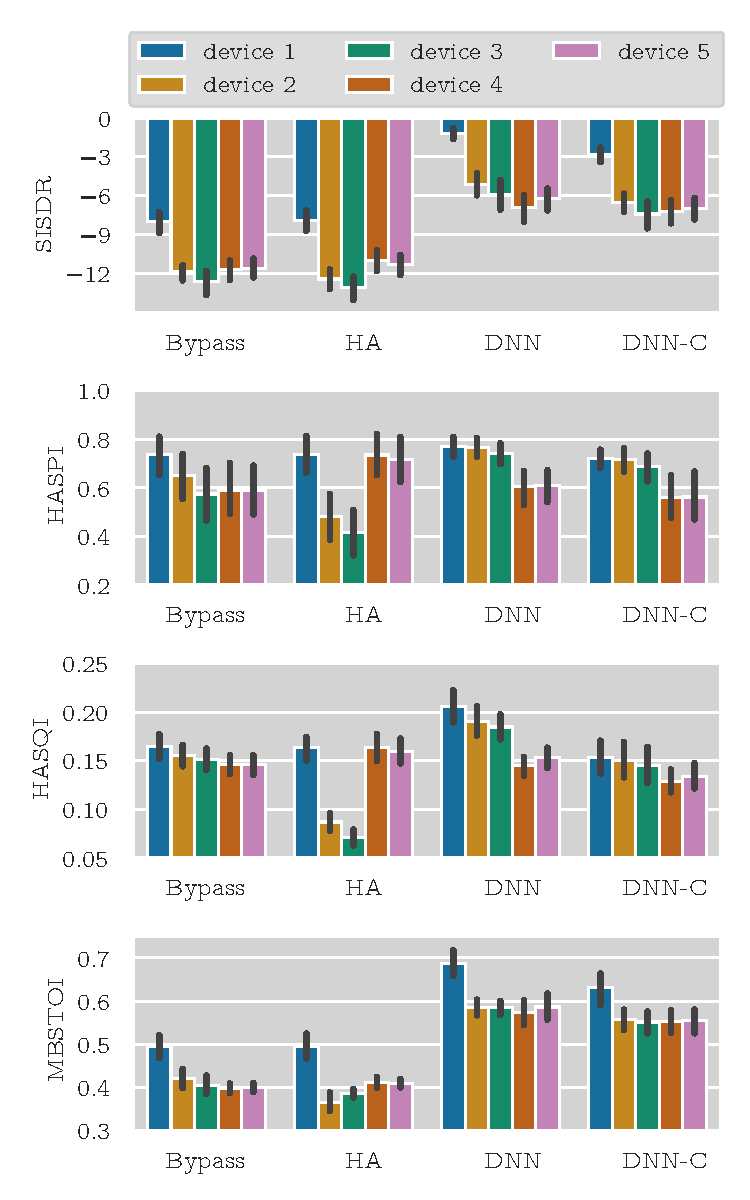
\includegraphics[width=0.7\columnwidth, trim={0cm 0cm 0cm 0.3cm},clip]{ch03_hearing/figures/results1.pdf}
  \caption{Objective metrics across devices, anonymized for avoiding any drawal of inappropriate interdevice conclusions.}
  \label{fig:ha_results1}
\end{figure}


Figure \ref{fig:ha_results2} depicts the signal enhancement benefit. Violin plots summarize the values obtained from the 15 hearing devices averaged along all scenes. For hearing aid features the benefit is on average 0.014 dB for SISDR, -0.02 for HASQI, -0.01 for HASPI, and -0.01 for MBSTOI. A much larger improvement could be observed for DNN-based enhancement. For a causal model, the mean benefit was 4.96 dB for SISDR, -0.01 for HASQI, 0.02 for HASPI, and 0.15 for MBSTOI. The largest benefit was achieved by the non-causal DNN model, with mean values reaching 6.09 dB for SISDR, 0.02 for HASQI, 0.07 for HASPI, and 0.17 for MBSTOI.


\begin{figure}[h!]
  \centering
  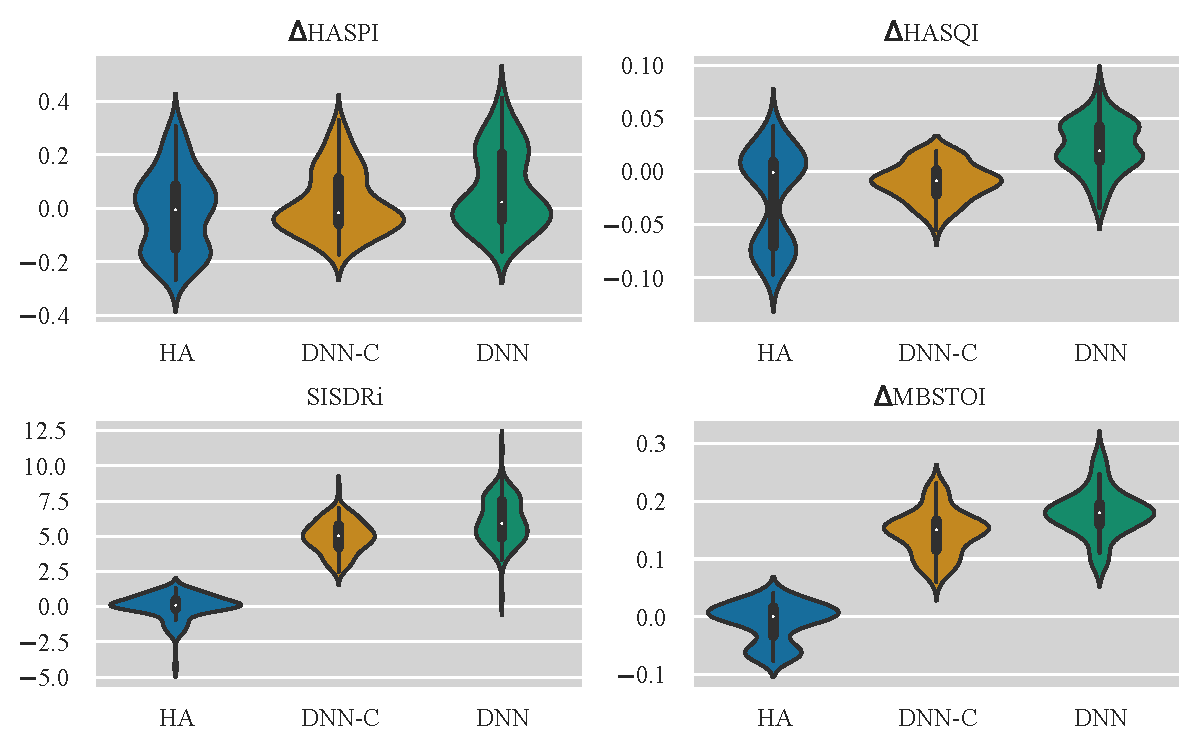
\includegraphics[width=\columnwidth, trim={0cm 0cm 0cm 0cm}]{ch03_hearing/figures/results2.pdf}
  \caption{Signal enhancement benefit for \acrshort{HAs}, non-causal \acrshort{DNN} model (DNN) and causal \acrshort{DNN} model (DNN-C). The corresponding mean values are collected in Table~\ref{tab:ha_benefit}.}
  \label{fig:ha_results2}
\end{figure}

\begin{table}[htbp]
\centering
\footnotesize
\caption{Mean signal enhancement benefit across the 15 \acrshort{HAs}-\acrshort{RIC} combinations,
averaged along all scenes, as depicted in Figure~\ref{fig:ha_results2}.}

\label{tab:ha_benefit}
\begin{tabular}{@{}lrrrr@{}}
\toprule
 & $SISDRi (dB) & $\Delta$HASQI & $\Delta$HASPI & $\Delta$MBSTOI \\
\midrule
HA    & $0.014$ & $-0.02$ & $-0.01$ & $-0.01$ \\
DNN-C & $4.96$  & $-0.01$ & $0.02$  & $0.15$  \\
DNN   & $6.09$  & $0.02$  & $0.07$  & $0.17$  \\
\bottomrule
\end{tabular}
\end{table}

\section{Discussion}
\label{sec:ha_discussion}

In this chapter we have presented a setup which allows to quantify the performance gap between the current hearing aid signal enhancement strategies and DNN-based approaches. On the one hand, HA processing seems to struggle in these complex situations, even performing worse than in \textit{bypass} for some devices, perhaps because beamformers cannot estimate the direction of the target speech due to the noise and competing talkers being non-stationary. On the other hand, this does not seem to affect DNNs, which improve SISDR and MBSTOI consistently. 

Interestingly, differences between devices in \textit{bypass} are still observed after being processed by the DNNs, suggesting that DNN models are sensitive to the quality of the inputs. It would be interesting to study the


\section{Conclusions}
\label{sec:ha_conclusions}

This chapter has shown that the signal-enhancement algorithms of five
high-end commercial \acrshort{HAs} struggle in ecologically valid, complex
acoustic situations reproduced in the studio, to the point of occasionally
degrading performance relative to applying no enhancement at all
(\textbf{RO1}). It has also shown that \acrshort{DNN}-based \acrfull{SE}
has the potential to outperform them substantially in denoising and objective
intelligibility (\textbf{RO2}), and that the causal
variant retains most
of that advantage. Together, these findings encourage further work on the
optimisation and pruning of such models for on-device deployment, and their
subjective validation with hearing-impaired listeners.

The evaluation presented here has since been complemented by a perceptual
study \citep{baig2025perceptual}, carried out by Mart\'i Baig as part of his
Master's thesis and therefore beyond the scope of this dissertation. Using the
same recordings and models, it ran a \acrshort{MUSHRA}-like listening test with
twenty hearing-aid users and twenty normal-hearing participants, and added a
\emph{mild} variant of both \acrshort{DNN}s, trained on pseudo-anechoic targets
so as to remove the noise while preserving some reverberation. Both groups
preferred the mild models over the hearing aids' own processing, and rated the
\emph{strong} variants studied in this chapter --- those trained on the fully
anechoic targets --- lowest of all, finding their noise suppression overly
aggressive and detrimental to naturalness and spatial perception. This
subjective evidence supports the objective findings reported above, while
suggesting that the anechoic target adopted here, discussed among the
limitations in Section~\ref{sec:ha_discussion}, is indeed more aggressive than
hearing-aid users would prefer.

Beyond the evaluation itself, the chapter contributes the infrastructure that
made it possible, released as research materials\footnote{\url{https://github.com/enricguso/guso_waspaa23}}: a set of \acrshort{HRTF}s
measured on a \acrshort{KU100} wearing a \acrshort{RIC} hearing aid, the
corresponding Ambisonics-to-binaural \acrshort{BiMagLS} decoder, a synthetic
binaural training corpus for \acrshort{HAs} \acrshort{SE}, and a reverberant
speech-in-noise test set in Ambisonic and binaural together with the
recordings of each device.